%%%%%%%%%%%%%%%%%%%%%%%%%%ch3-3
\begin{frame}[shrink]
  \frametitle{ch3.信号检测与估计理论的基础知识}
  \framesubtitle{ch3-3. 派生贝叶斯准则(2),信号统计检测的性能及M元信号的统计检测}
  \tableofcontents[hideallsubsections]
\end{frame}

\section{极小极大化准则(续)}

\begin{frame}[shrink]{极小极大化准则}
给定$P_{1g}$的条件下, 平均代价$C(P_1,P_{1g})$是先验概率$P_1$的线性函数, 若$P_{1g}\ne P_1$, 平均代价$C(P_1,P_{1g})$大于最小平均代价。\\
为避免产生过分大的代价, 需要猜测一种先验概率$P_{1g}^\ast$, 使得平均代价$C(P_1,P_{1g}^\ast)$不依赖于信源的先验概率$P_1$。
\begin{columns}
	\column{0.7\textwidth}
	\begin{align*}
	&C(P_1,P_{1g})=c_{00}+(c_{10}-c_{00})P_F(P_{1g})+\\
	&P_1[(c_{11}-c_{00})+(c_{01}-c_{11})P_M(P_{1g})-(c_{10}-c_{00})P_F(P_{1g})]\\
	&\frac{\partial C(P_1,P_{1g})}{\partial P_1}\left|_{P_{1g}=P_{1g}^\ast}\right.=0\\
	&\textbf{\textcolor{blue}{极小化极大方程}}\\
	&(c_{11}-c_{00})+(c_{01}-c_{11})P_M(P_{1g}^\ast)-(c_{10}-c_{00})P_F(P_{1g}^\ast)=0
	\end{align*}
	\column{0.3\textwidth}
	\centering
	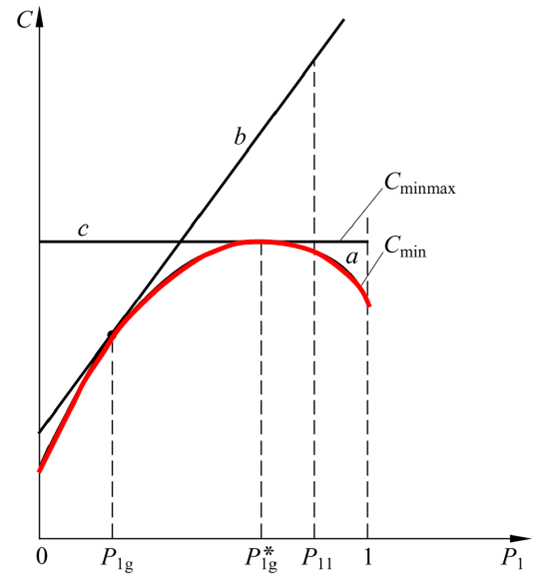
\includegraphics[scale=0.25]{C-P1}
\end{columns}
~\\
\textbf{\textcolor{blue}{平均代价: }} $C(P_{1g}^\ast)=c_{00}+(c_{10}-c_{00})P_F(P_{1g}^\ast)$
\end{frame}

\begin{frame}[shrink]{极小极大化准则}
\textbf{\textcolor{blue}{极小化极大方程}}
\[(c_{11}-c_{00})+(c_{01}-c_{11})P_M(P_{1g}^\ast)-(c_{10}-c_{00})P_F(P_{1g}^\ast)=0 \]
\textbf{\textcolor{blue}{平均代价: }} \[C(P_{1g}^\ast)=c_{00}+(c_{10}-c_{00})P_F(P_{1g}^\ast) \]
\begin{block}{正确判决不付出代价}
\begin{columns}
	\column{0.3\textwidth}
	$c_{11}=c_{00}=0$
	\column{0.5\textwidth}
	$c_{01}P_M(P_{1g}^\ast)=c_{10}P_F(P_{1g}^\ast)$ 
\end{columns}
\end{block}
\begin{block}{正确判决不付出代价, 错误判决代价因子相同}
\begin{columns}
	\column{0.3\textwidth}
	$c_{11}=c_{00}=0$\\
	$c_{10}=c_{01}=1$
	\column{0.5\textwidth}
	$P_M(P_{1g}^\ast)=P_F(P_{1g}^\ast)$ 
\end{columns}
\end{block}
\end{frame}

\begin{frame}{极小化极大准则的基本步骤}
\begin{enumerate}
\setlength{\itemsep}{.5cm}
\item 计算两个似然函数, 构建似然比$\lambda(x)\mathop{=}\limits^{def}\frac{p(x|H_1)}{p(x|H_0)}$
\item 假设判决门限$\eta$, 构建贝叶斯检测基本表达式
\item 化简成最简形式$l(x)\mathop{\gtrless}\limits_{H_0}^{H_1}\gamma(\eta)$
\item 利用极小化极大准则, 确定最终判决门限$\gamma(\eta)$
\end{enumerate}
\end{frame}

\begin{frame}{贝叶斯准则例题6}
在闭启键控通信系统中,两个假设下的观测信号模型为:
\begin{align*}
H_0: x&=n  \\
H_1: x&=A+n
\end{align*}
其中, 噪声$n$是均值为零,方差为$\sigma_n^2$的高斯噪声,  若两个假设的先验概率未知, 且$c_{00}=c_{11}=0, c_{01}=c_{10}=1$。\\
~\\
采用极小化极大准则,试确定检测门限, 并求最小平均错误概率。
\end{frame}

\begin{frame}[shrink]{贝叶斯准则例题6: 解}
解: 观测信号模型为:
\begin{align*}
H_0: x&=n  \\
H_1: x&=A+n
\end{align*}
\textbf{步骤1: 计算两个似然函数, 构建似然比}\\
由于$n$是高斯分布随机变量, 因此在$H_0$假设下, 检测统计量$x$服从高斯分布,且均值为0, 方差为$\sigma_n^2$; 在$H_1$假设下, 检测统计量$x$服从均值为$A$, 方差为$\sigma_n^2$的高斯分布。
\begin{align*}
&p(x|H_0)=\left(\frac{1}{2\pi\sigma_n^2}\right)^{1/2}\exp\left(-\frac{x^2}{2\sigma_n^2}\right) \qquad p(x|H_1)=\left(\frac{1}{2\pi\sigma_n^2}\right)^{1/2}\exp\left(-\frac{(x-A)^2}{2\sigma_n^2}\right)\\
&\lambda(x)=\frac{p(x|H_1)}{p(x|H_0)}=\exp\left(\frac{(x^2-(x-A)^2)}{2\sigma_n^2}\right)=\exp\left(\frac{A}{\sigma_n^2}x-\frac{A^2}{2\sigma_n^2}\right)
\end{align*} 
\end{frame}

\begin{frame}[shrink]{贝叶斯准则例题6: 解(续1)}
\textbf{步骤2: 假设判决门限$\eta$, 构建贝叶斯检测基本表达式}
\begin{align*}
&\lambda(x)\mathop{=}^{def}\frac{p(x|H_1)}{p(x|H_0)}\mathop{\gtrless}_{H_0}^{H_1}\eta\\
&\lambda(x)=\exp\left(\frac{A}{\sigma_n^2}x-\frac{A^2}{2\sigma_n^2}\right)
\end{align*} 
\textbf{步骤3: 化简成最简形式}
\begin{align*}
&x\mathop{\gtrless}_{H_0}^{H_1}\frac{\sigma_n^2\ln\eta}{A}+\frac{A}{2}\mathop{=}^{def}\gamma
\end{align*} 
\end{frame}

\begin{frame}[shrink]{贝叶斯准则例题6: 解(续2)}
\textbf{步骤4: 利用极小化极大准则, 确定最终判决门限$\gamma$}
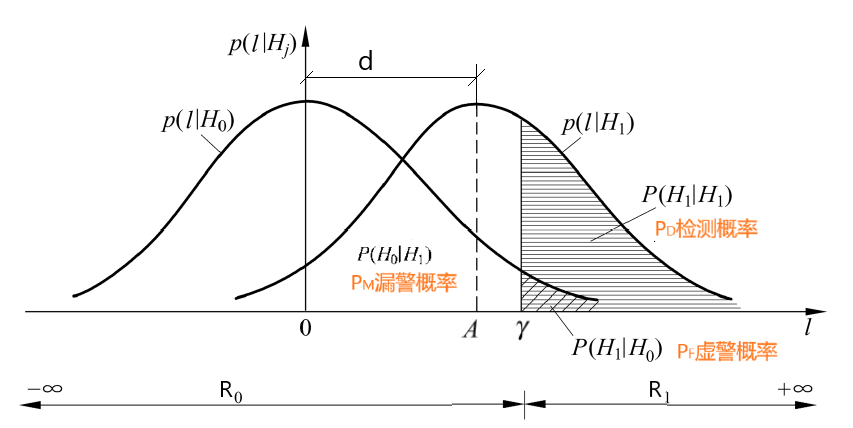
\includegraphics[scale=0.3]{R0R1}
\begin{align*}
P_F\mathop{=}^{def}P(H_1|H_0)&=\int_{\gamma}^{\infty}p(x|H_0)dx\implies Q(x)=\int_{x}^{\infty}\left(\frac{1}{2\pi}\right)^{1/2}\exp\left(-\frac{u^2}{2}\right)du\\
&=\int_{\gamma}^{\infty}\left(\frac{1}{2\pi\sigma_n^2}\right)^{1/2}\exp\left(-\frac{x^2}{2\sigma_n^2}\right)dx\qquad \text{by } x=\sigma_nu\\
&=\int_{\frac{\gamma}{\sigma_n}}^{\infty}\left(\frac{1}{2\pi}\right)^{1/2}\exp\left(-\frac{u^2}{2}\right)du\\
&=Q\left(\frac{\gamma}{\sigma_n}\right)
\end{align*}
\end{frame}

\begin{frame}[shrink]{贝叶斯准则例题6: 解(续3)}
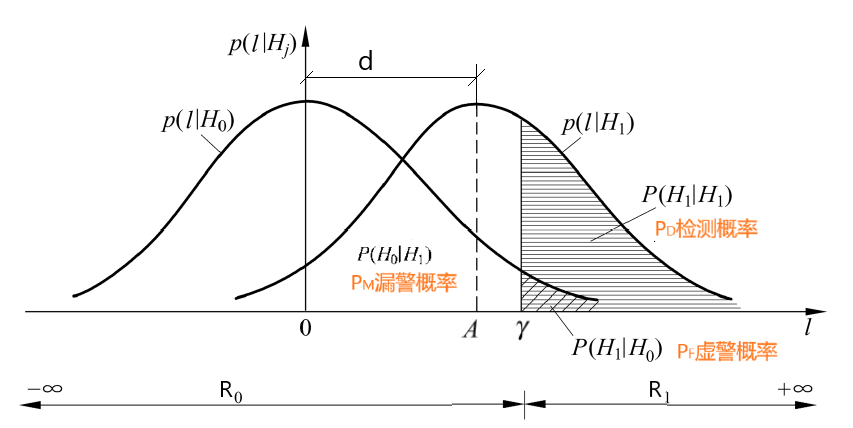
\includegraphics[scale=0.3]{R0R1}
\begin{align*}
P_M\mathop{=}^{def}P(H_0|H_1)&=1-\int_{\gamma}^{\infty}p(x|H_1)dx\implies Q(x)=\int_{x}^{\infty}\left(\frac{1}{2\pi}\right)^{1/2}\exp\left(-\frac{u^2}{2}\right)du\\
&=1-\int_{\gamma}^{\infty}\left(\frac{1}{2\pi\sigma_n^2}\right)^{1/2}\exp\left(-\frac{(x-A)^2}{2\sigma_n^2}\right)dx\qquad \text{by } x=\sigma_nu+A\\
&=1-\int_{\frac{\gamma-A}{\sigma_n}}^{\infty}\left(\frac{1}{2\pi}\right)^{1/2}\exp\left(-\frac{u^2}{2}\right)du\\
&=1-Q\left(\frac{\gamma-A}{\sigma_n}\right)
\end{align*}
\end{frame}

\begin{frame}[shrink]{贝叶斯准则例题6: 解(续4)}
\begin{block}{正确判决不付出代价, 错误判决代价因子相同时的极小化极大方程}
\begin{columns}
\column{0.3\textwidth}
$c_{11}=c_{00}=0$\\
$c_{10}=c_{01}=1$
\column{0.5\textwidth}
$P_M(P_{1g}^\ast)=P_F(P_{1g}^\ast)$ 
\end{columns}
\end{block}
\begin{columns}[T]
\column{0.5\textwidth}
\small
\begin{align*}
P_F\mathop{=}^{def}P(H_1|H_0)&=Q\left(\frac{\gamma}{\sigma_n}\right)\\
P_M\mathop{=}^{def}P(H_0|H_1)&=1-Q\left(\frac{\gamma-A}{\sigma_n}\right)\\
&=Q\left(-\frac{\gamma-A}{\sigma_n}\right)
\end{align*}
根据上述极小化极大方程,有
\begin{align*}
Q\left(\frac{\gamma}{\sigma_n}\right)=Q\left(-\frac{\gamma-A}{\sigma_n}\right)\implies \gamma=\frac{A}{2}
\end{align*}
\column{0.5\textwidth}
\small
\begin{align*}
&Q(x)=\int_{x}^{\infty}\left(\frac{1}{2\pi}\right)^{1/2}\exp\left(-\frac{u^2}{2}\right)du\\
&Q\left(\frac{d}{2}\right) = 1-Q\left(-\frac{d}{2}\right)
\end{align*}
\centering
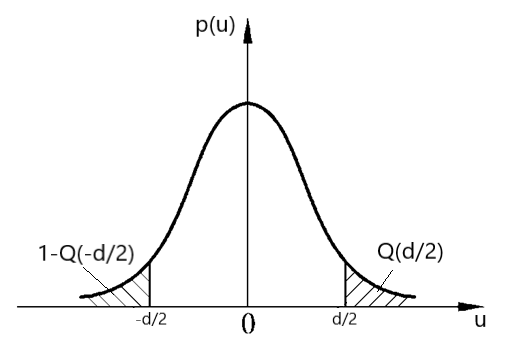
\includegraphics[scale=0.25]{Qdd}
\end{columns}
\end{frame}

\begin{frame}[shrink]{贝叶斯准则例题6: 解(续5)}
\small
\textbf{本例, 按照极小化极大准则,平均错误概率为:}
\begin{align*}
P_e&=P(H_1)P(H_0|H_1)+P(H_0)P(H_1|H_0)\\
&=P(H_1)P_M+P(H_0)P_F\\
&=[P(H_1)+P(H_0)]P_F &&\text{by 本例的极小化极大方程}P_M(P_{1g}^\ast)=P_F(P_{1g}^\ast)\\
&=P_F=P(H_1|H_0) &&\text{by }P(H_1)+P(H_0)=1, P_F\mathop{=}^{def}P(H_1|H_0)\\
&=Q(\frac{\gamma}{\sigma})=Q\left(\frac{A}{2\sigma}\right) && \text{by }\gamma=\frac{A}{2}\\
&=Q(\frac{d}{2}) &&\text{by 功率信噪比}d^2=\frac{A^2}{\sigma^2}
\end{align*}
\textbf{例题5, 按照按照平均错误概率准则,平均错误概率同上。}\\
因此, \textbf{\textcolor{blue}{先验等概条件下的最小平均错误准则等价于正确判决为0, 错误判决代价为1时的极小化极大准则。}}
\end{frame}

\section{奈曼---皮尔逊准则}

\begin{frame}[shrink]{奈曼---皮尔逊准则(Neyman-Pearson criterion)}
\begin{columns}
\column{0.72\textwidth}
\begin{itemize}
%\setlength{\itemsep}{.5cm}
\item \textbf{\textcolor{blue}{应用范围}}\\
假设的先验概率未知, 判决代价未知(雷达信号检测)
\item \textbf{\textcolor{blue}{目标}}\\
错误判决概率尽可能小, 正确判决概率尽可能大
\item \textbf{\textcolor{blue}{实际情况}}\\
$P(H_1|H_0)$减小时, $P(H_1|H_1)$也相应减小;\\
增加$P(H_1|H_1)$, $P(H_1|H_0)$也随之增加。
\item \textbf{\textcolor{blue}{奈曼皮尔逊检测}}\\
在虚警概率$P_F\mathop{=}\limits^{def}P(H_1|H_0)=\alpha$约束条件下, 使正确判决概率(检测概率)$P_D\mathop{=}\limits^{def}P(H_1|H_1)$最大的准则。
\end{itemize}
\column{0.28\textwidth}
\leftline{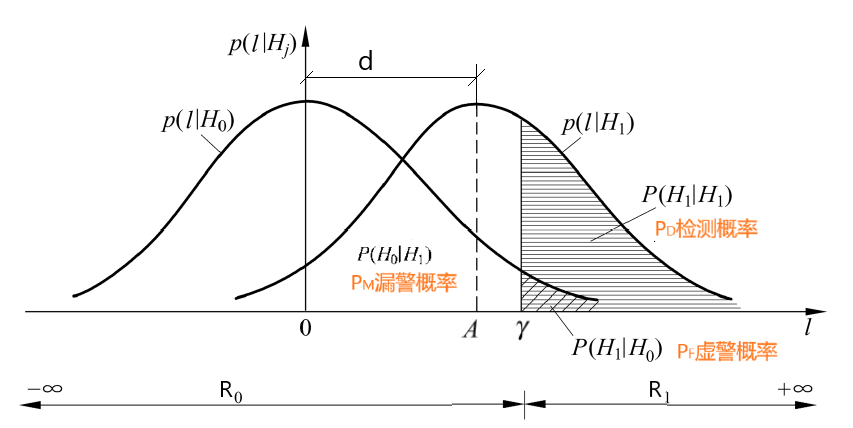
\includegraphics[scale=0.17]{R0R1}}
\end{columns}
\end{frame}

\begin{frame}{奈曼---皮尔逊准则的存在性}
\begin{columns}
\column{0.5\textwidth}
\begin{enumerate}
\item 图中,三个判决域$(R_{0i},R_{1i})$均满足错误判决概率$P_i(H_1|H_0)=\alpha(i=0,1,2)$。
\item 原则上判决域$R_0$和$R_1$有无限多种划分方法,均可以保证错误判决概率$P(H_1|H_0)=\alpha$, 但是正确判决概率$P(H_1|H_1)$一般是不一样的。
\item 至少有一种判决域划分能使$P(H_1|H_0)=\alpha$,又能使$P(H_1|H_1)$到达最大。
\end{enumerate}
\column{0.4\textwidth}
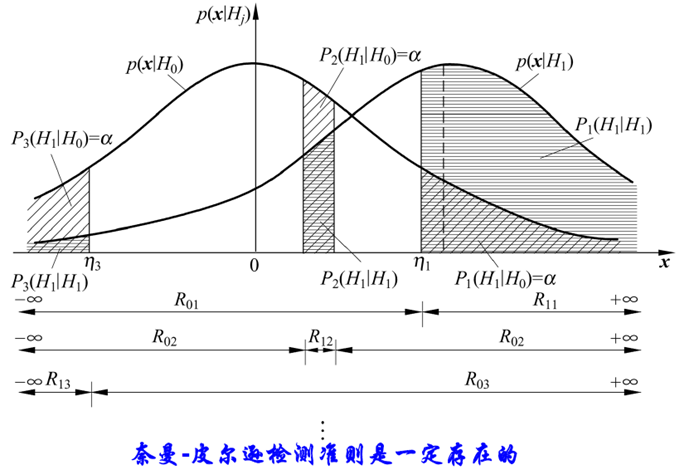
\includegraphics[scale=0.45]{Neyman-Pearson}
\end{columns}
\end{frame}

\begin{frame}[shrink]{奈曼---皮尔逊准则的推导}
在$P(H_1|H_0)=\alpha$约束条件下, 使正确判决概率$P(H_1|H_1)$最大的准则\\
\qquad\qquad\qquad $\Updownarrow$\quad(由于$P(H_0|H_1)+P(H_1|H_1)=1$)\\
在$P(H_1|H_0)=\alpha$约束条件下, 使错误判决概率$P(H_0|H_1)$最小的准则
\rule{\textwidth}{1pt} %水平线
利用拉格朗日乘子$\mu(\mu\ge 0)$, 构建目标函数
\[ J=P(H_0|H_1)+\mu\left[P(H_1|H_0)-\alpha\right]\]
若$P(H_1|H_0)=\alpha, J$达到最小时, $P(H_0|H_1)$也达到最小。
\begin{columns}
\scriptsize
\column{0.5\textwidth}
漏警概率$P(H_0|H_1)+$检测概率$P(H_1|H_1)=1$,\\ 虚警概率$P(H_1|H_0)=\alpha$\\
当$J$最小$\implies$漏警概率$(P(H_0|H_1)$最小\\
$\implies$检测概率$P(H_1|H_1)$最大。
\column{0.5 \textwidth}
\leftline{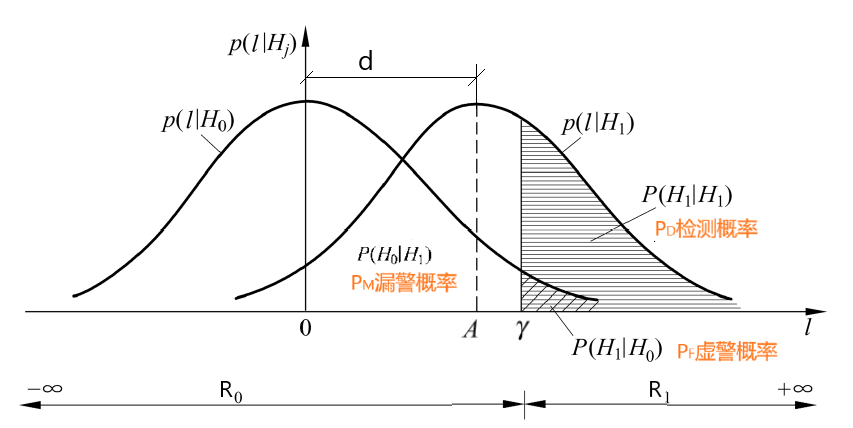
\includegraphics[scale=0.25]{R0R1}}
\end{columns}
\end{frame}

\begin{frame}[shrink]{奈曼---皮尔逊准则的推导(续)}
\begin{columns}
\column{0.4\textwidth}
\begin{align*}
J&=P(H_0|H_1)+\mu[P(H_1|H_0)-\alpha]\\
&=\int_{R_0}p(x|H_1)dx+\mu\left[\int_{R_1}p(x|H_0)dx-\alpha\right]\\
&=\int_{R_0}p(x|H_1)dx+\mu\left[1-\int_{R_0}p(x|H_0)dx-\alpha\right]\\
&=\mu(1-\alpha)+\int_{R_0}\left[p(x|H_1)-\mu p(x|H_0)\right]dx \\
\end{align*}
\column{0.4\textwidth}
\leftline{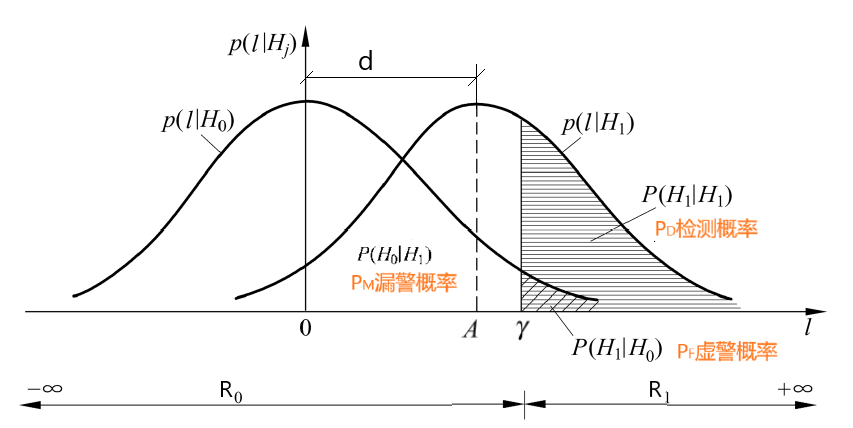
\includegraphics[scale=0.23]{R0R1}}
\end{columns}
\textbf{\textcolor{blue}{把使被积函数取负值的观测值$x$值划分给$R_0$区域, 而把其余的观测值$x$值划分给$R_1$, 即可保证平均代价最小, 从而使$J$值最小。}}
\begin{align*}
&p(x|H_1)< \mu p(x|H_0)&\textbf{判决$H_0$假设成立}\\
&p(x|H_1)\ge \mu p(x|H_0)&\textbf{判决$H_1$假设成立}
\end{align*}
\end{frame}

\begin{frame}[shrink]{奈曼---皮尔逊准则}
\begin{block}{奈曼---皮尔逊准则}
\[ \lambda(x)\mathop{=}\limits^{def}\frac{p(x|H_1)}{p(x|H_0)}\mathop{\gtrless}_{H_0}^{H_1}\mu \]
其中, 判决门限有下式确定
\begin{align*}
P(H_1|H_0)=\int_{R_1}p(x|H_0)dx=\int_{\mu}^{\infty}p(\lambda|H_0)d\lambda=\alpha\
\end{align*}
求出的$\mu$必满足$\mu\ge 0$
\end{block}
\begin{block}{贝叶斯判决准则}
\[ \lambda(x)=\frac{p(x|H_1)}{p(x|H_0)}\mathop{\gtrless}_{H_0}^{H_1}\frac{P(H_0)(c_{10}-c_{00})}{P(H_1)(c_{01}-c_{11})}\mathop{=}^{def}\eta \]
\end{block}
贝叶斯准则的特例, 当$P(H_1)(c_{01}-c_{11})=1, P(H_0)(c_{10}-c_{00})=\mu$时, 就成为奈曼---皮尔逊准则。
\end{frame}

\begin{frame}[shrink]{奈曼---皮尔逊准则的求解步骤}
\begin{enumerate}
\setlength{\itemsep}{.5cm}
\item 计算两个似然函数, 构建似然比$\lambda(x)\mathop{=}\limits^{def}\frac{p(x|H_1)}{p(x|H_0)}\mathop{\gtrless}\limits_{H_0}^{H_1}\mu$
\item 假设判决门限$\mu$, 构建贝叶斯检测基本表达式
\item 化简
\item 根据统计量计算$p(l|H_0)$和$p(l|H_1)$
\item 在$P(H_1|H_0)=\int_{R_1}p(l|H_0)dl=\alpha$约束下, 计算判决门限
\end{enumerate}
\end{frame}

\begin{frame}{贝叶斯准则例题7}
在闭启键控通信系统中,两个假设下的观测信号模型为:
\begin{align*}
H_0: x&=n  \\
H_1: x&=1+n
\end{align*}
其中, 噪声$n$是均值为零,方差为1的高斯噪声。\\
~\\
试构造在$P(H_1|H_0)=0.1$条件下的奈曼---皮尔逊接收机
\end{frame}

\begin{frame}[shrink]{贝叶斯准则例题7: 解}
解: 观测信号模型为:
\begin{align*}
H_0: x&=n  \\
H_1: x&=1+n
\end{align*}
\textbf{步骤1: 计算两个似然函数, 构建似然比}\\
由于$n$是高斯分布随机变量, 因此在$H_0$假设下, 检测统计量$x$服从高斯分布,且均值为0, 方差为$\sigma_n^2$; 在$H_1$假设下, 检测统计量$x$服从均值为$1$, 方差为$\sigma_n^2$的高斯分布。
\begin{align*}
&p(x|H_0)=\left(\frac{1}{2\pi\sigma_n^2}\right)^{1/2}\exp\left(-\frac{x^2}{2\sigma_n^2}\right) \qquad p(x|H_1)=\left(\frac{1}{2\pi\sigma_n^2}\right)^{1/2}\exp\left(-\frac{(x-1)^2}{2\sigma_n^2}\right)\\
&\lambda(x)=\frac{p(x|H_1)}{p(x|H_0)}=\exp\left(\frac{(x^2-(x-1)^2)}{2\sigma_n^2}\right)=\exp\left(\frac{1}{\sigma_n^2}x-\frac{1}{2\sigma_n^2}\right)
\end{align*} 
\end{frame}

\begin{frame}[shrink]{贝叶斯准则例题7: 解(续1)}
\textbf{步骤2: 假设判决门限$\mu$, 构建贝叶斯检测基本表达式}
\begin{align*}
&\lambda(x)\mathop{=}^{def}\frac{p(x|H_1)}{p(x|H_0)}\mathop{\gtrless}_{H_0}^{H_1}\mu\\
&\lambda(x)=\exp\left(\frac{1}{\sigma_n^2}x-\frac{1}{2\sigma_n^2}\right)
\end{align*} 
\textbf{步骤3: 化简成最简形式}
\begin{align*}
&x\mathop{\gtrless}_{H_0}^{H_1}\sigma_n^2\ln\mu+\frac{1}{2}\mathop{=}^{def}\gamma\\
&\text{by }\sigma_n=1\\
&x\mathop{\gtrless}_{H_0}^{H_1}\ln\mu+\frac{1}{2}\mathop{=}^{def}\gamma\\
\end{align*} 
\end{frame}

\begin{frame}[shrink]{贝叶斯准则例题7: 解(续2)}
\textbf{步骤4: 利用奈曼---皮尔逊准则, 确定最终判决门限$\gamma$}
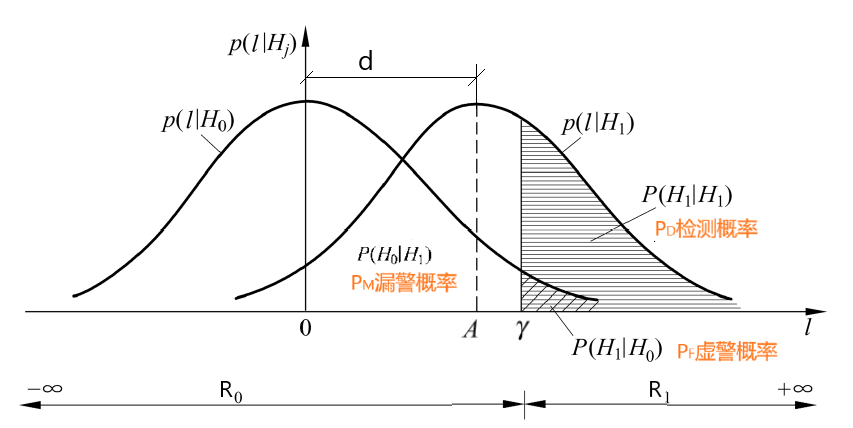
\includegraphics[scale=0.3]{R0R1}
\begin{align*}
P_F\mathop{=}^{def}P(H_1|H_0)&=\int_{\gamma}^{\infty}p(x|H_0)dx\implies Q(x)=\int_{x}^{\infty}\left(\frac{1}{2\pi}\right)^{1/2}\exp\left(-\frac{u^2}{2}\right)du\\
&=\int_{\gamma}^{\infty}\left(\frac{1}{2\pi\sigma_n^2}\right)^{1/2}\exp\left(-\frac{x^2}{2\sigma_n^2}\right)dx\qquad \text{by } x=\sigma_nu\\
&=\int_{\frac{\gamma}{\sigma_n}}^{\infty}\left(\frac{1}{2\pi}\right)^{1/2}\exp\left(-\frac{u^2}{2}\right)du\\
&=Q\left(\frac{\gamma}{\sigma_n}\right)=Q(\gamma)\qquad \text{by }\sigma_n=1
\end{align*}
\end{frame}

\begin{frame}[shrink]{贝叶斯准则例题7: 解(续3)}
\begin{columns}
\column{0.55\textwidth}
\begin{align*}
&x\mathop{\gtrless}_{H_0}^{H_1}\ln\mu+\frac{1}{2}\mathop{=}^{def}\gamma\\
&P(H_1|H_0)=Q(\gamma)
\end{align*} 
在$P(H_1|H_0)=0.1$条件下,确定判决门限\\
由$Q(\gamma)=0.1$, 解得$\gamma=1.29$,\\
由$\ln\mu+\frac{1}{2}=\gamma$, 解得$\mu=2.2$
\column{0.4\textwidth}
\leftline{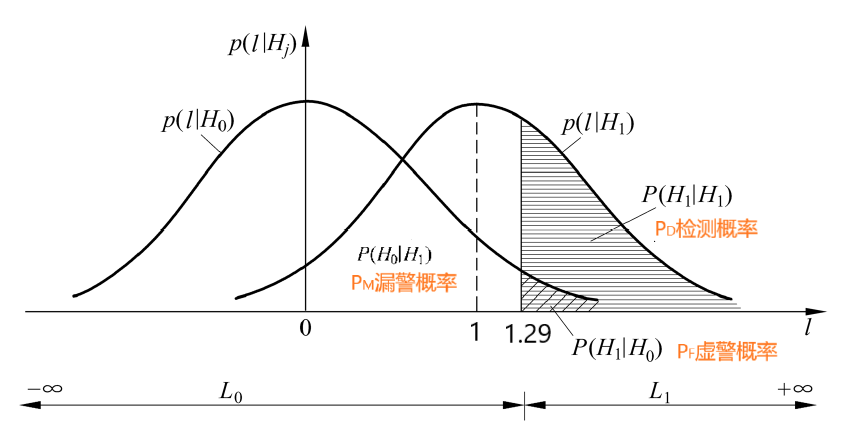
\includegraphics[scale=0.3]{ex3-7}}
\end{columns}
\begin{align*}
P_D\mathop{=}^{def}P(H_1|H_1)&=\int_{\gamma}^{\infty}p(x|H_1)dx\implies Q(x)=\int_{x}^{\infty}\left(\frac{1}{2\pi}\right)^{1/2}\exp\left(-\frac{u^2}{2}\right)du\\
&=\int_{\gamma}^{\infty}\left(\frac{1}{2\pi\sigma_n^2}\right)^{1/2}\exp\left(-\frac{(x-1)^2}{2\sigma_n^2}\right)dx\qquad \text{by } x=\sigma_nu+1\\
&=\int_{\frac{\gamma-1}{\sigma_n}}^{\infty}\left(\frac{1}{2\pi}\right)^{1/2}\exp\left(-\frac{u^2}{2}\right)du\\
&=Q\left(\frac{\gamma-1}{\sigma_n}\right)=Q(\gamma-1)=Q(0.29)=0.386
\end{align*}
\end{frame}

\begin{frame}[shrink]{贝叶斯准则以及派生贝叶斯准则(1)}
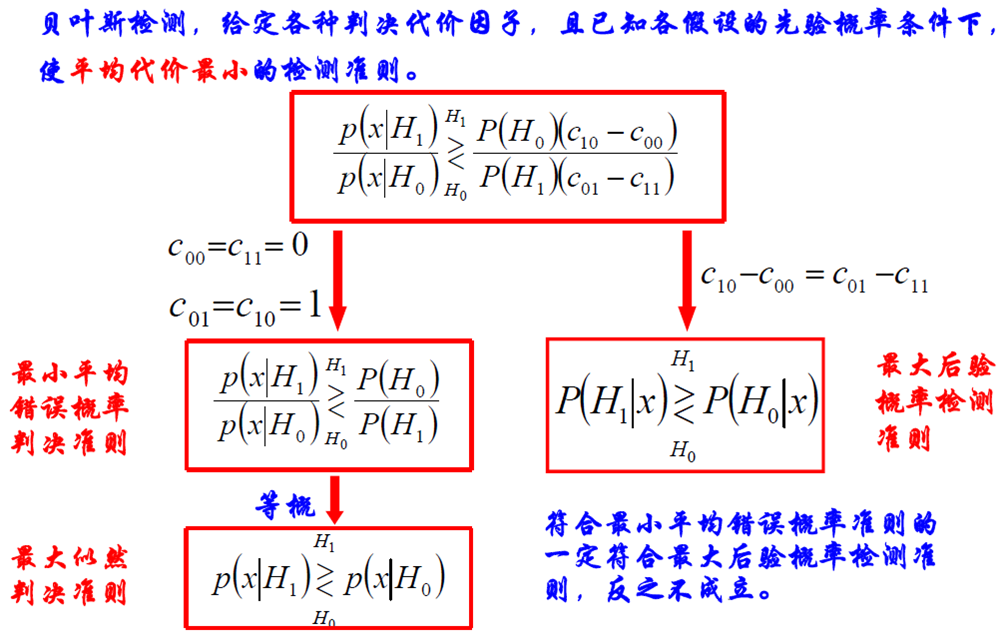
\includegraphics[scale=0.5]{bys}
\end{frame}

\begin{frame}[shrink]{贝叶斯准则以及派生贝叶斯准则(2)}
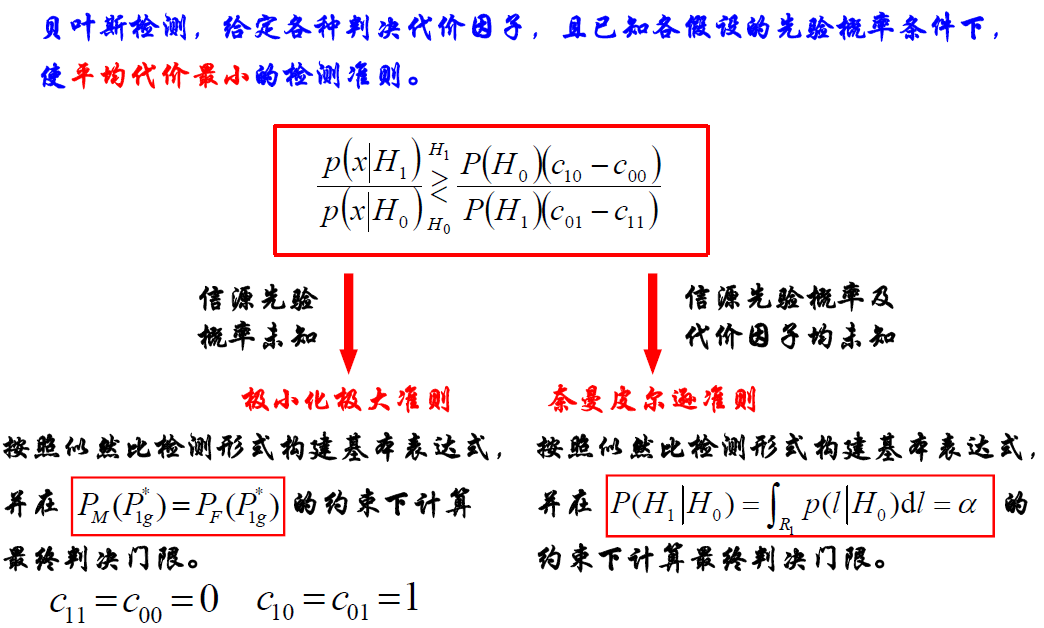
\includegraphics[scale=0.5]{bys2}
\end{frame}

\begin{frame}[shrink]{贝叶斯准则以及派生贝叶斯准则求解步骤}
分析某种检测方法得性能时,需要根据化简后得最简判决表示式进行。\\
计算步骤:\\
\begin{enumerate}
%\setlength{\itemsep}{.5cm}
\item 推导某种检测方法下获得的最简判决表达式$l(x)\mathop{\gtrless}\limits_{H_0}^{H_1}\gamma$
\item 根据最简表示式, 计算各种假设下, 统计量的概率密度函数
\[p(l|H_0)\qquad p(l|H_1) \]
\item 计算判决概率\\
\[P(H_0|H_1)\qquad P(H_1|H_0) \]
\end{enumerate}
\end{frame}

\begin{frame}{信号统计检测的性能}
\begin{block}{基本要求}
	\begin{itemize} \setstretch{2.5}
		\item 理解判决概率的不同计算方法
		\item 理解似然比检测的接收机工作特性
		\item 利用接收机工作特性求解不同检测准则的解	
	\end{itemize}
\end{block}
\end{frame}

\section{信号统计检测的性能}

\begin{frame}[shrink]{信号统计检测的性能}
\begin{itemize}
	\item \textbf{\textcolor{blue}{判决概率计算}}
		\begin{align*}
		&\lambda(\bm{x})=\frac{p(\bm{x}|H_1)}{p(\bm{x}|H_0)}\mathop{\gtrless}_{H_0}^{H_1}\eta && l(\bm{x}) \mathop{\gtrless}_{H_0}^{H_1}\gamma\\
		&P(H_1|H_0)=\int_{\eta}^{\infty}p(\lambda|H_0)d\lambda && P(H_1|H_0)=\int_{\gamma}^{\infty}p(l|H_0)dl\\
		&P(H_1|H_1)=\int_{\eta}^{\infty}p(\lambda|H_1)d\lambda && P(H_1|H_1)=\int_{\gamma}^{\infty}p(l|H_1)dl
		\end{align*}
	\item \textbf{\textcolor{blue}{似然比检测的接收机工作特性}}\\
根据$P_D=P(H_1|H_1)$和$P_F=P(H_1|H_0)$分析似然比检测的接收机工作特性
\end{itemize}
\rightline{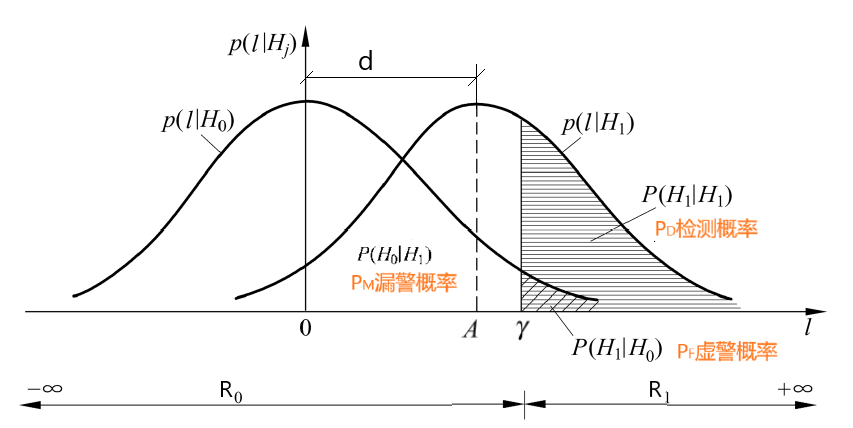
\includegraphics[scale=0.25]{R0R1}}
\end{frame}

\begin{frame}[shrink]{信号统计检测的性能}
\begin{itemize}
	\item \textbf{\textcolor{blue}{判决概率计算}}
	\begin{align*}
	&\lambda(\bm{x})=\frac{p(\bm{x}|H_1)}{p(\bm{x}|H_0)}\mathop{\gtrless}_{H_0}^{H_1}\eta && l(\bm{x}) \mathop{\gtrless}_{H_0}^{H_1}\gamma\\
	&P(H_1|H_0)=\int_{\eta}^{\infty}p(\lambda|H_0)d\lambda && P(H_1|H_0)=\int_{\gamma}^{\infty}p(l|H_0)dl\\
	&P(H_1|H_1)=\int_{\eta}^{\infty}p(\lambda|H_1)d\lambda && P(H_1|H_1)=\int_{\gamma}^{\infty}p(l|H_1)dl
	\end{align*}
	\item \textbf{\textcolor{blue}{似然比检测的接收机工作特性}}\\
	根据$P_D=P(H_1|H_1)$和$P_F=P(H_1|H_0)$分析似然比检测的接收机工作特性
\end{itemize}
\rightline{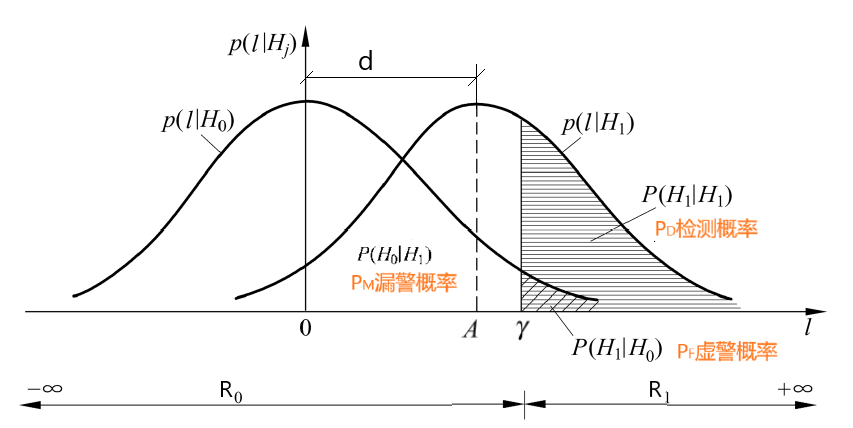
\includegraphics[scale=0.25]{R0R1}}
\end{frame}

\begin{frame}[shrink]{例如, 雷达信号检测}
\begin{columns}
\column{0.21\textwidth}
$H_0:x_k=n_k$\\
$H_1:x_k=A+n_k$
\column{0.79\textwidth}
\[
\frac{1}{N}\sum\limits_{k=1}^{N}x_k\mathop{\gtrless}\limits_{H_0}^{H_1}\frac{\sigma_n^2\ln\eta}{NA}+\frac{A}{2}\mathop{=}\limits^{def}\gamma \qquad \textbf{统计量: }l(\bm{x})\mathop{=}\limits^{def}\frac{1}{N}\sum\limits_{k=1}^{N}x_k
\]
\end{columns}
\textbf{假设$H_0$条件下, 统计量$l(x)$为高斯分布, $(l|H_0)\sim\mathcal{N}(0,\frac{\sigma_n^2}{N})$}
\begin{align*}
p(l|H_0)=\left(\frac{N}{2\pi\sigma_n^2}\right)^{1/2}\exp\left(-\frac{Nl^2}{2\sigma_n^2}\right)
\end{align*}
\textbf{假设$H_1$条件下, 统计量$l(x)$为高斯分布, $(l|H_1)\sim\mathcal{N}(A,\frac{\sigma_n^2}{N})$}
\begin{align*}
p(l|H_1)=\left(\frac{N}{2\pi\sigma_n^2}\right)^{1/2}\exp\left(-\frac{N(l-A)^2}{2\sigma_n^2}\right)
\end{align*}
\end{frame}

\begin{frame}[shrink]{虚警概率$P_F=P(H_1|H_0)$}
\begin{align*}
P(H_1|H_0)&=\int_{\gamma}^{\infty}p(l|H_0)dl\implies Q(x)=\int_{x}^{\infty}\left(\frac{1}{2\pi}\right)^{1/2}\exp\left(-\frac{u^2}{2}\right)du\\
&=\int_{\gamma}^{\infty}\left(\frac{N}{2\pi\sigma_n^2}\right)^{1/2}\exp\left(-\frac{Nl^2}{2\sigma_n^2}\right)dl\qquad \text{by } l=\frac{\sigma_nu}{\sqrt{N}}\\
&=\int_{\frac{\sqrt{N}\gamma}{\sigma_n}}^{\infty}\left(\frac{1}{2\pi}\right)^{1/2}\exp\left(-\frac{u^2}{2}\right)du\\
&=Q\left(\frac{\sqrt{N}\gamma}{\sigma_n}\right) &&\text{by } \gamma=\frac{\sigma_n^2\ln\eta}{NA}+\frac{A}{2}\\
&=Q\left(\frac{\sqrt{N}\left(\frac{\sigma_n^2\ln\eta}{NA}+\frac{A}{2}\right)}{\sigma_n}\right)\\
&=Q\left(\frac{\sigma_n\ln\eta}{\sqrt{N}A}+\frac{\sqrt{N}A}{2\sigma_n}\right) &&\text{by }d^2=\frac{NA^2}{\sigma_n^2}\\
&=Q\left(\frac{\ln\eta}{d}+\frac{d}{2}\right)
\end{align*}
\end{frame}

\begin{frame}[shrink]{检测概率$P_D=P(H_1|H_1)$}
\begin{align*}
P(H_1|H_1)&=\int_{\gamma}^{\infty}p(l|H_1)dl\implies Q(x)=\int_{x}^{\infty}\left(\frac{1}{2\pi}\right)^{1/2}\exp\left(-\frac{u^2}{2}\right)du\\
&=\int_{\gamma}^{\infty}\left(\frac{N}{2\pi\sigma_n^2}\right)^{1/2}\exp\left(-\frac{N(l-A)^2}{2\sigma_n^2}\right)dl\qquad \text{by } l=\frac{\sigma_nu}{\sqrt{N}}+A\\
&=\int_{\frac{\sqrt{N}(\gamma-A)}{\sigma_n}}^{\infty}\left(\frac{1}{2\pi}\right)^{1/2}\exp\left(-\frac{u^2}{2}\right)du\\
&=Q\left(\frac{\sqrt{N}(\gamma-A}{\sigma_n}\right) &&\text{by } \gamma=\frac{\sigma_n^2\ln\eta}{NA}+\frac{A}{2}\\
&=Q\left(\frac{\sqrt{N}\left(\frac{\sigma_n^2\ln\eta}{NA}-\frac{A}{2}\right)}{\sigma_n}\right)\\
&=Q\left(\frac{\sigma_n\ln\eta}{\sqrt{N}A}-\frac{\sqrt{N}A}{2\sigma_n}\right)&& \text{by }d^2=\frac{NA^2}{\sigma_n^2}\\
&=Q\left(\frac{\ln\eta}{d}-\frac{d}{2}\right)
\end{align*}
\end{frame}

\begin{frame}[shrink]{判决域与判决概率}
\begin{columns}
\column{0.6\textwidth}
$N$次独立采样, 样本为$x_k(k=1,2,\dots,N)$
\begin{align*}
&&n_k\sim\mathcal{N}(0,\sigma_n^2)\\ 
H_0 &:x_k=n_k   &(l|H_0)\sim\mathcal{N}(0,\frac{\sigma_n^2}{N})\\
H_1 &:x_k=A+n_k &(l|H_1)\sim\mathcal{N}(A,\frac{\sigma_n^2}{N})
\end{align*}
检验统计量$l(\bm{x})$, 归一化后, $(l|H_j)\sim\mathcal{N}(0,1)$
\column{0.4\textwidth}
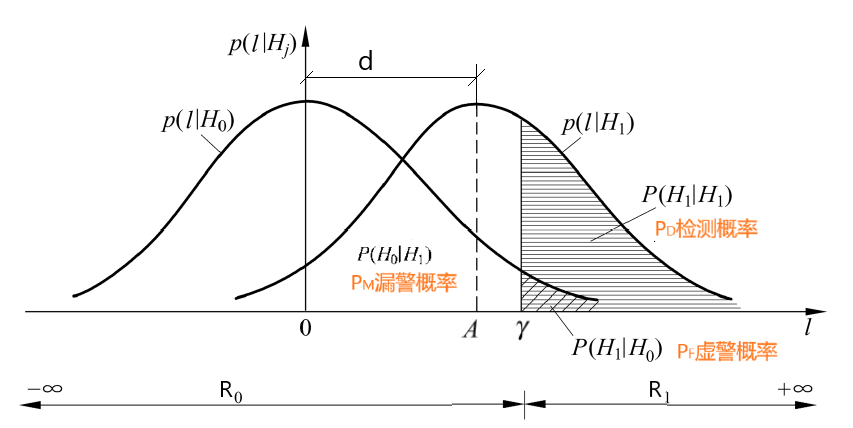
\includegraphics[scale=0.28]{R0R1}\\
\end{columns}
\[
\textbf{判决表达式: }\qquad l(\bm{x})\mathop{=}^{def}\frac{1}{N}\sum\limits_{k=1}^Nx_k\mathop{\gtrless}_{H_0}^{H_1}\frac{\sigma^2\ln\eta}{NA}+\frac{A}{2}\mathop{=}^{def}\gamma
\]

\textbf{判决概率:} (式中, 信噪比$d^2=\frac{NA^2}{\sigma_n^2}$)
\begin{align*}
\textbf{虚警概率: }P_F\mathop{=}^{def}P(H_1|H_0)&=Q\left(\frac{\ln\eta}{d}+\frac{d}{2}\right)\\
\textbf{检测概率: }P_D\mathop{=}^{def}P(H_1|H_1)&=Q\left(\frac{\ln\eta}{d}-\frac{d}{2}\right)
\end{align*}
\end{frame}

\begin{frame}[shrink]{接收机工作特性}
\begin{columns}[T]
	\column{0.6\textwidth}
	\begin{itemize}
		\small
		\item 错误判别概率(虚警概率):
		\[P_F\mathop{=}^{def}P(H_1|H_0)=Q\left(\frac{\ln\eta}{d}+\frac{d}{2}\right)\]
		\item 正确判别概率(检测概率):
		\[P_D\mathop{=}^{def}P(H_1|H_1)=Q\left(\frac{\ln\eta}{d}-\frac{d}{2}\right)\]
		\item 不同的信噪比$d$, 有不同的$P_D\sim P_F$曲线
		\item 似然比函数$\lambda(x)$超过无穷大门限$\eta=+\infty$是不可能事件, $(P_D,P_F)=(0,0)$
		\item $\lambda(x)\ge 0$, $\eta=0$是必然事件, $(P_D,P_F)=(1,1)$
		\item 当$\lambda(x)$是连续随机变量时, $\eta\uparrow\implies (P_D,P_F)\downarrow$
	\end{itemize}
	\column{0.4\textwidth}
	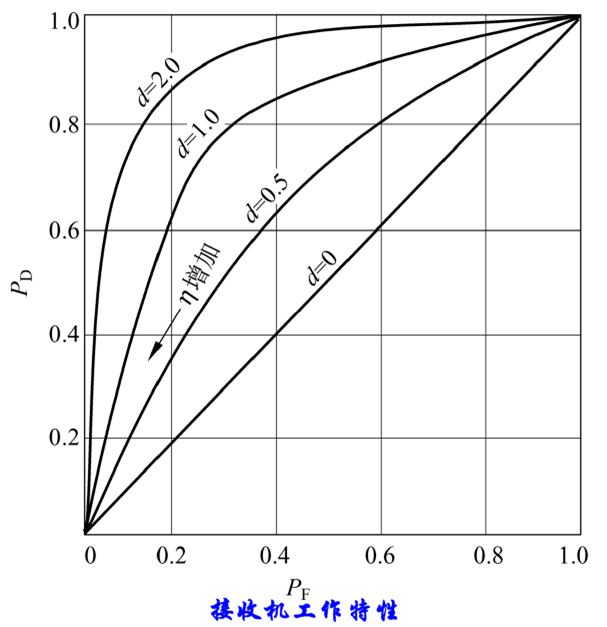
\includegraphics[scale=0.28]{PDPF}\\
	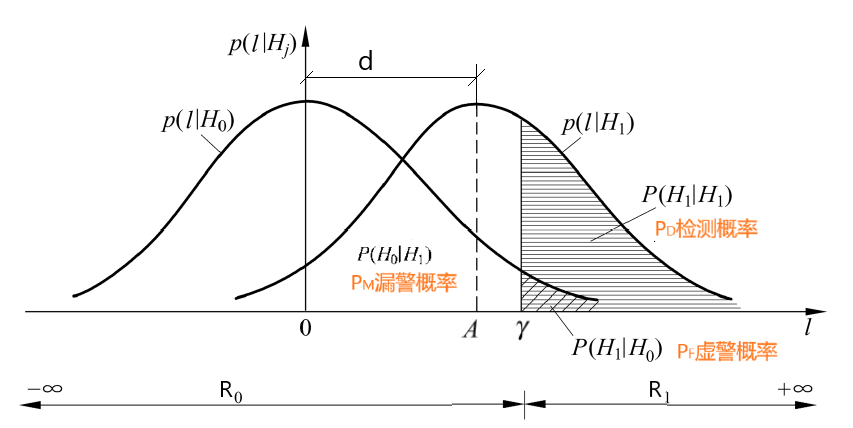
\includegraphics[scale=0.2]{R0R1}
\end{columns}
\end{frame}

\begin{frame}[shrink]{接收机工作特性的共同特点}
\begin{columns}[T]
	\column{0.6\textwidth}
	\begin{itemize}
		\small
		\item 上凸曲线
		\item 曲线位于$P_D=P_F$之上
		\item 随着门限$\eta$的增加, 两种判决概率$P_D$和$P_F$之都会减小
		\item $P_D$和$P_F$同时增加,或同时减小
		\item 给定$P_D(P_F)$, 随着信噪比$d$的增加, $P_F$减小($P_D$增加)
		\item 工作特性某点上的斜率等于该点$P_D$和$P_F$所要求的检测门限值
		\item 利用接收机工作特性,可进行各种判决准则的分析和计算
	\end{itemize}
	\column{0.4\textwidth}
	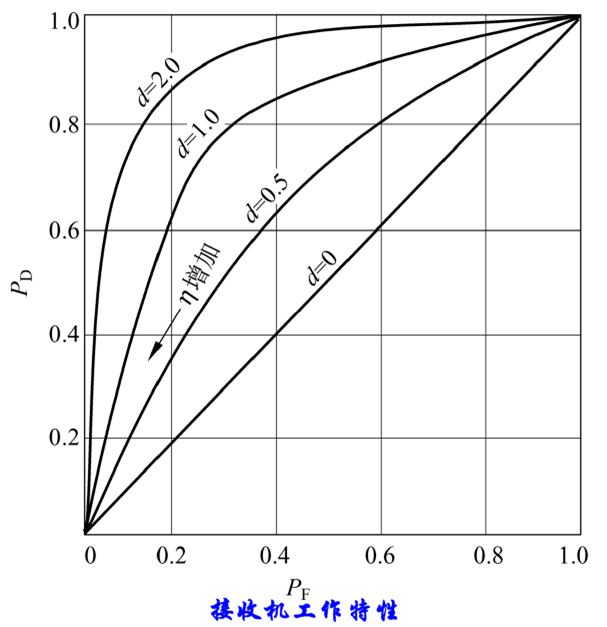
\includegraphics[scale=0.28]{PDPF}\\
	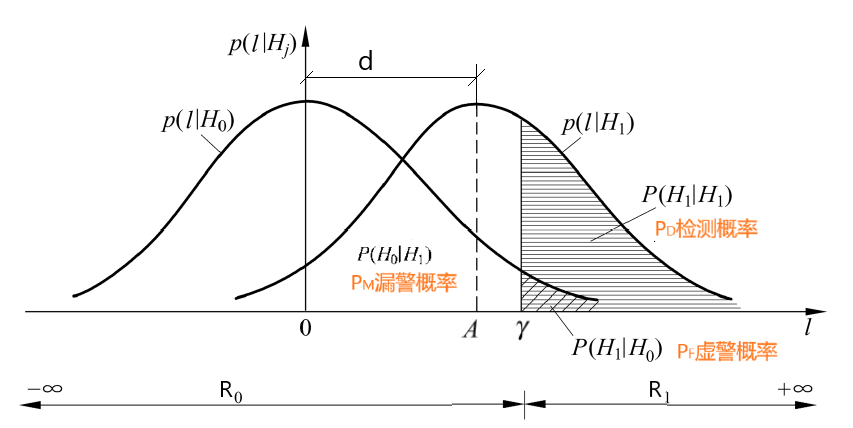
\includegraphics[scale=0.2]{R0R1}
\end{columns}
\end{frame}

\begin{frame}[shrink]{检测概率$P_D$与信噪比$d$的关系}
信噪比$d$是接收机的主要指标之一,因此常把接收机工作特性改成$P_D\sim d$曲线, 而以$P_F$作为参变量。
\begin{columns}
	\column{0.5\textwidth}
	\begin{align*}
	P_F&=P(H_1|H_0)=Q(\ln\eta/d+d/2)\\ 
	&\ln\eta/d=Q^{-1}[P(H_1|H_0)]-d/2\\
	P_D&=P(H_1|H_1)=Q\left(\ln\eta/d-d/2\right)\\
	&=Q[Q^{-1}[P(H_1|H_0)]-d/2-d/2]\\
	&=Q[Q^{-1}[P(H_1|H_0)]-d]
	\end{align*}
	\column{0.5\textwidth}
	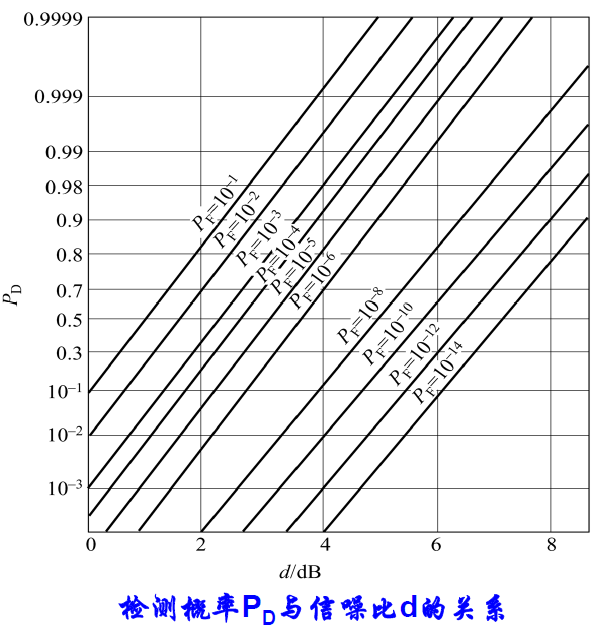
\includegraphics[scale=0.5]{PD-d}
\end{columns}

\medskip

\colorbox{yellow}{$Q(x)$是递减函数, 当给定$P_F$时, $P_D$随功率信噪比$(d^2=NA^2/\sigma_n^2)$单调增加。} 
\end{frame}

\begin{frame}[shrink]{工作特性某点上的斜率等于该点$P_D$和$P_F$所要求的检测门限值$\eta$}
\begin{columns}
	\column{0.5\textwidth}
	\begin{align*}
	&P_D\mathop{=}^{def}P(H_1|H_1)=\int_{\eta}^{\infty}p(\lambda|H_1)d\lambda\mathop{=}^{def}P_D(\eta) \\
	&P_F\mathop{=}^{def}P(H_1|H_0)=\int_{\eta}^{\infty}p(\lambda|H_0)d\lambda\mathop
	{=}^{def}P_F(\eta) \\
	&\frac{dP_D(\eta)}{d\eta} =-p(\eta|H_1) \\ 
	&\frac{dP_F(\eta)}{d\eta} =-p(\eta|H_0) \\ 
	&\qquad \text{ by } \Phi^\prime(x)=\frac{d}{dx}\int_a^xf(t)dt=f(x)\qquad (a\le x\le b) \\
	&\frac{dP_D(\eta)}{dP_F(\eta)} =\frac{-p(\eta|H_1)}{-p(\eta|H_0)}=\frac{p(\eta|H_1)}{p(\eta|H_0)}
	\end{align*}
	\column{0.5\textwidth}
	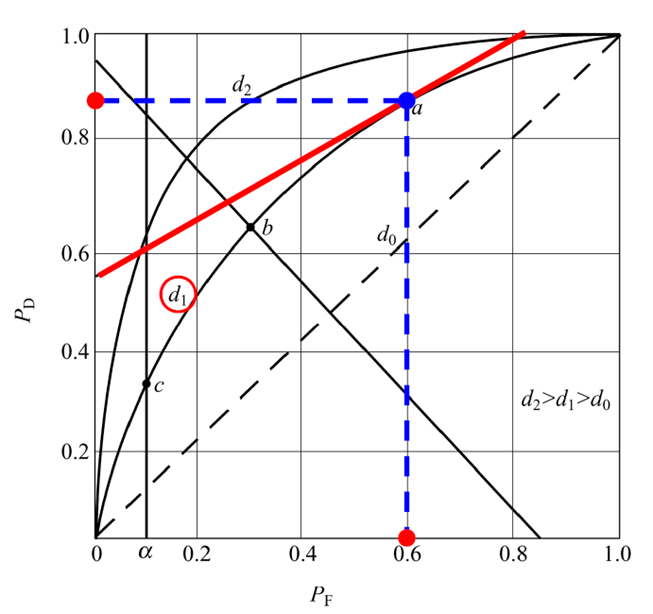
\includegraphics[scale=0.48]{PD-PF-e}
\end{columns}
\end{frame}

\begin{frame}[shrink]{工作特性某点上的斜率等于该点$P_D$和$P_F$所要求的检测门限值$\eta$}
\begin{columns}[T]
	\column{0.5\textwidth}
	\small
	\begin{align*}
	P_D(\eta) &=P[(\lambda|H_1)\ge\eta]&\\
	&=\int_{\eta}^{\infty}p(\lambda|H_1)d\lambda=\int_{R_1}^{\infty}p(x|H_1)dx&\\
	&=\int_{R_1}^{\infty}\lambda p(x|H_0)dx \qquad \text{ by }\lambda(x)=\frac{p(x|H_1)}{p(x|H_0)}\mathop{\gtrless}_{H_0}^{H_1}\eta&\\
	&=\int_{\eta}^{\infty}\lambda p(\lambda|H_0)d\lambda&\\
	&\text{ by } \Phi^\prime(x)=\frac{d}{dx}\int_a^xf(t)dt=f(x)\qquad (a\le x\le b) \\
	\frac{dP_D(\eta)}{d\eta} &=-\eta p(\eta|H_0)\\
	\frac{dP_D(\eta)}{dP_F(\eta)} &=\frac{-p(\eta|H_1)}{-p(\eta|H_0)}=\frac{-\eta p(\eta|H_0)}{-p(\eta|H_0)}=\eta
	\end{align*}
	\column{0.5\textwidth}
	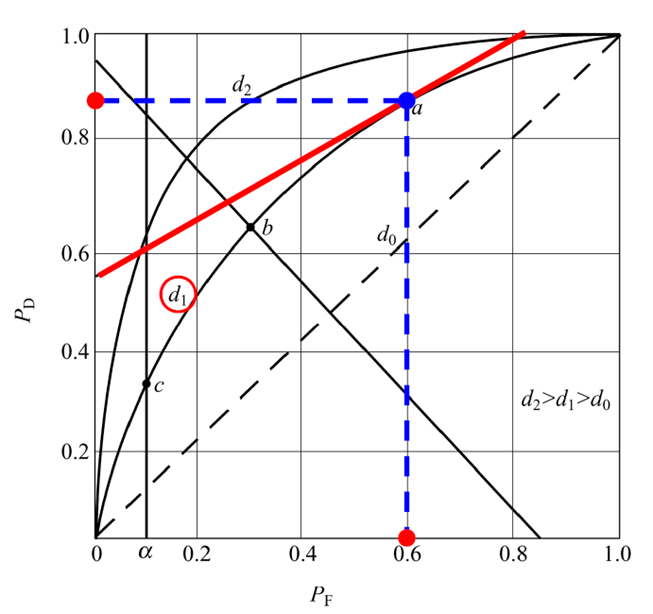
\includegraphics[scale=0.47]{PD-PF-e}
\end{columns}\end{frame}

\section{利用接收机工作特性,各种判决准则的分析和计算}

\begin{frame}[shrink]{贝叶斯准则和最小错误概率准则}
\begin{columns}[T]
	\column{0.5\textwidth}
		\begin{itemize}
		\item 根据先验概率和代价因子, 求得判决门限$\eta$
		\item 以$\eta$为斜率, 可找到一条直线, 与在给定信噪比$d$下的$P_D-P_F$曲线相切; 如, $d=d_1$, 切点$u$
		\item 切点对应的$P_D$和$P_F$值,就是在给定信噪比下的两种判决概率。
	\end{itemize}
	\column{0.5\textwidth}
	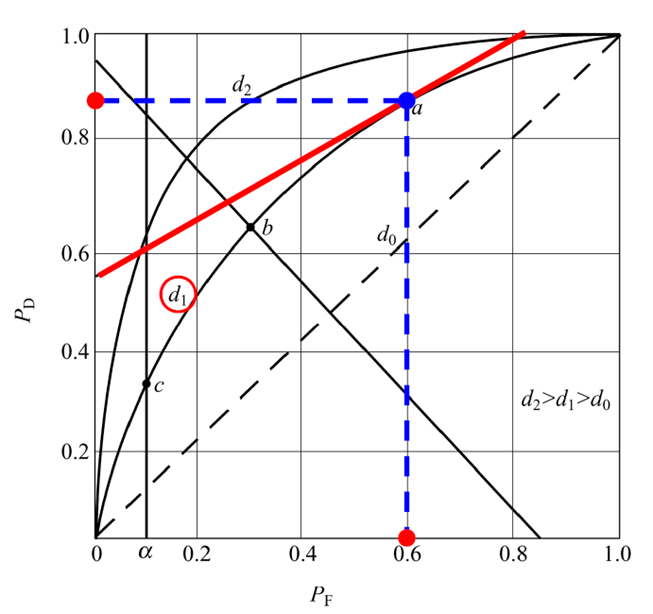
\includegraphics[scale=0.5]{PD-PF-e}
\end{columns}
\end{frame}

\begin{frame}[shrink]{极小化极大准则}
\textbf{\textcolor{blue}{满足极小化极大方程}}
\begin{align*}
&(c_{11}-c_{00})+(c_{01}-c_{11})P_M(P_{1g}^\ast)-(c_{10}-c_{00})P_F(P_{1g}^\ast)=0\\
&(c_{11}-c_{00})+(c_{01}-c_{11})\left(1-P_D(P_{1g}^\ast)\right)-(c_{10}-c_{00})P_F(P_{1g}^\ast)=0\\
&(c_{01}-c_{11})P_D(P_{1g}^\ast)+(c_{10}-c_{00})P_F(P_{1g}^\ast)-c_{01}+c_{00}=0
\end{align*}
\begin{columns}[T]
	\column{0.5\textwidth}
	\begin{align*}
	&P_D \mathop{=}^{def}P_F(P_1)=P(H_1|H_1)\\
	&P_F \mathop{=}^{def}P_F(P_1)=P(H_1|H_0)\\
	&P_M \mathop{=}^{def}P_M(P_1)=P(H_0|H_1)=1-P_D\\
	&P_M(P_{1g}^\ast)=1-P_D(P_{1g}^\ast)
	\end{align*}
	\[\bm{P_M(P_{1g}^\ast)=1-P_D(P_{1g}^\ast)} \]
	\column{0.5\textwidth}
	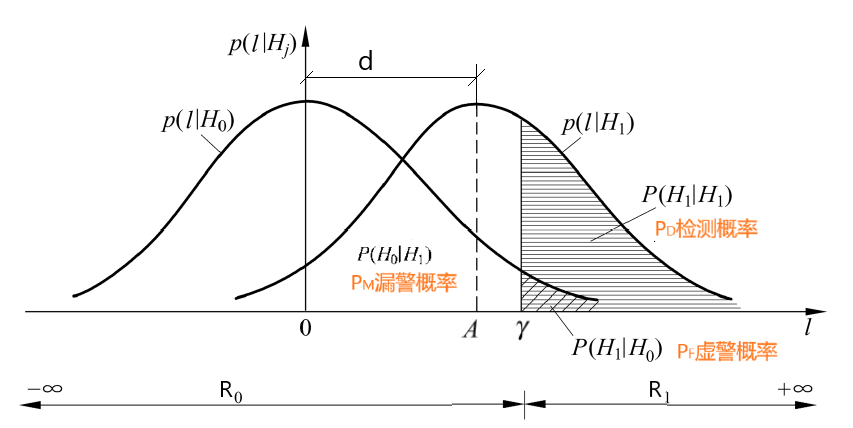
\includegraphics[scale=0.25]{R0R1}
\end{columns}
\end{frame}

\begin{frame}[shrink]{极小化极大准则}
\begin{columns}[T]
	\column{0.5\textwidth}
	\begin{itemize}
		\item 按照满足极小化极大方程的关系公式,画出一条$P_D-P_F$直线, 该直线与给定信噪比下的$P_D-P_F$工作特性曲线相交。如, $d=d_1$, 交点$b$
		\item 交点即是在极小化极大准则条件下的两种判决概率。
	\end{itemize}
	\column{0.5\textwidth}
	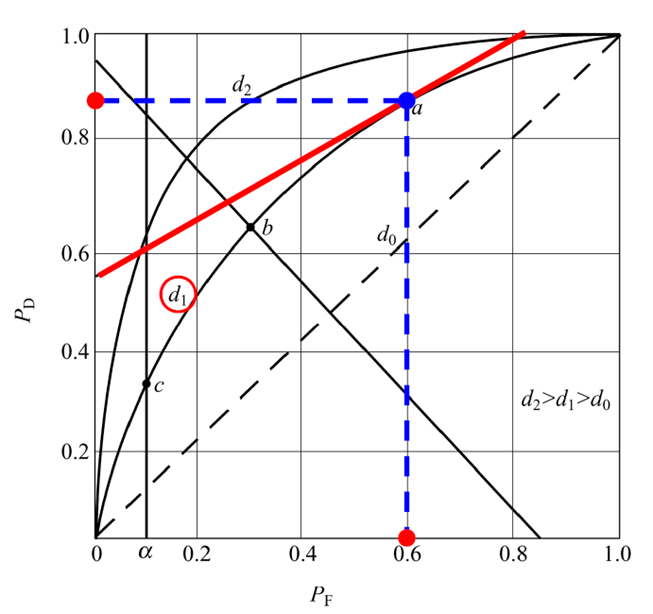
\includegraphics[scale=0.5]{PD-PF-e}
\end{columns}
\textbf{\textcolor{blue}{满足极小化极大方程}}
\begin{align*}
(c_{01}-c_{11})P_D(P_{1g}^\ast)+(c_{10}-c_{00})P_F(P_{1g}^\ast)-c_{01}+c_{00}=0
\end{align*}
\end{frame}

\begin{frame}[shrink]{奈曼---皮尔逊准则}
\begin{columns}[T]
	\column{0.5\textwidth}
	\begin{itemize}
		\item 由$P_F=\alpha$画一条直线
		\item 该直线与给定信噪比下的$P_D-P_F$工作特性曲线相交。如, $d=d_1$, 交点$c$
		\item 交点即是在奈曼---皮尔逊准则下的两种判决概率。
	\end{itemize}
	\column{0.5\textwidth}
	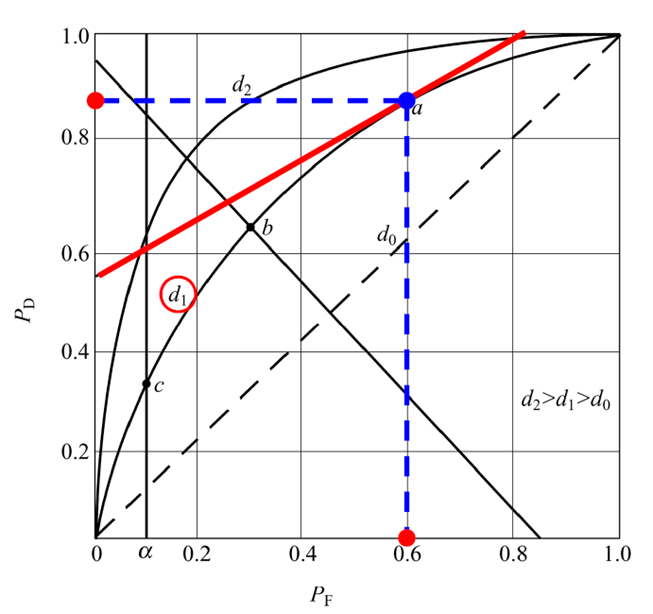
\includegraphics[scale=0.5]{PD-PF-e}
\end{columns}
\end{frame}

\section{M元信号的统计检测}

\begin{frame}{M元信号的统计检测}
\begin{block}{基本要求}
	\begin{itemize} \setstretch{2.5}
		\item 了解贝叶斯准则
		\item 了解最小平均错误概率准则和最大似然准则
	\end{itemize}
\end{block}
\end{frame}

\begin{frame}{M元信号检测检测模型}
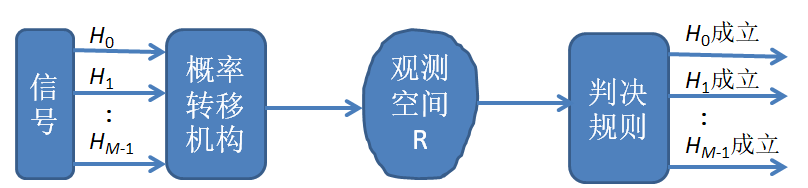
\includegraphics[scale=0.4]{M}
\newline
\begin{columns}
	\column{0.4\textwidth}
	判决域划分:
	\[\bm{R}=\bigcup_{i=0}^{M-1}R_i, R_i\cap R_j=\emptyset, (i\ne j) \]
	\column{0.6\textwidth}
	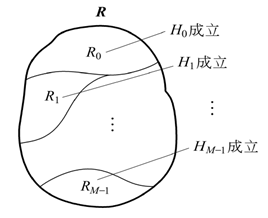
\includegraphics[scale=0.4]{R-M}
\end{columns}
\end{frame}

\begin{frame}[shrink]{贝叶斯准则}
给定各假设先验概率及各判决代价因子。问题: 寻找一种判决空间的划分方法, 使平均代价最小。\\
\textbf{平均代价: }
\begin{align*}
C&=P(H_0)C(H_0)+P(H_1)C(H_1)\\
C(H_0)&=c_{00}P(H_0|H_0)+c_{10}P(H_1|H_0)\\
C(H_1)&=c_{01}P(H_0|H_1)+c_{11}P(H_1|H_1)\\
C=&P(H_0)(c_{00}P(H_0|H_0)+c_{10}P(H_1|H_0))+\\
&P(H_1)(c_{01}P(H_0|H_1)+c_{11}P(H_1|H_1))
\end{align*}
\centering$\Downarrow$
\[
C=\sum_{i=0}^{M-1}\sum_{j=0}^{M-1}c_{ij}P(H_j)P(H_i|H_j)
\]
\end{frame}

\begin{frame}[shrink]{平均代价计算}
\begin{align*}
C&=\sum_{i=0}^{M-1}\sum_{j=0}^{M-1}c_{ij}P(H_j)P(H_i|H_j)\\
&=\sum_{i=0}^{M-1}c_{ii}P(H_i)P(H_i|H_i)+\sum_{i=0}^{M-1}\sum_{j=0,j\ne i}^{M-1}c_{ij}P(H_j)P(H_i|H_j)\\
&\quad \text{by } P(H_i|H_i)=1-\sum_{j=0,j\ne i}^{M-1}P(H_j|H_i)\\
&=\sum_{i=0}^{M-1}c_{ii}P(H_i)\left(1-\sum_{j=0,j\ne i}^{M-1}P(H_j|H_i)\right)+\sum_{i=0}^{M-1}\sum_{j=0,j\ne i}^{M-1}c_{ij}P(H_j)P(H_i|H_j)\\
&=\sum_{i=0}^{M-1}c_{ii}P(H_i)-\sum_{i=0}^{M-1}\sum_{j=0,j\ne i}^{M-1}c_{ii}P(H_i)P(H_j|H_i)+\sum_{i=0}^{M-1}\sum_{j=0,j\ne i}^{M-1}c_{ij}P(H_j)P(H_i|H_j)\\
\end{align*}
\end{frame}

\begin{frame}[shrink]{平均代价计算}
\begin{align*}
&\text{因为 }\quad \sum_{i=0}^{M-1}\sum_{j=0}^{M-1}c_{ii}P(H_i)P(H_j|H_i)=\sum_{i=0}^{M-1}\sum_{j=0}^{M-1}c_{jj}P(H_j)P(H_i|H_j)\\
&\text{所以 }\quad \sum_{i=0}^{M-1}\sum_{j=0,j\ne i}^{M-1}c_{ii}P(H_i)P(H_j|H_i)=\sum_{i=0}^{M-1}\sum_{j=0,j\ne i}^{M-1}c_{jj}P(H_j)P(H_i|H_j)
\end{align*}
\begin{align*}
C&=\sum_{i=0}^{M-1}c_{ii}P(H_i)-\sum_{i=0}^{M-1}\sum_{j=0,j\ne i}^{M-1}c_{ii}P(H_i)P(H_j|H_i)+\sum_{i=0}^{M-1}\sum_{j=0,j\ne i}^{M-1}c_{ij}P(H_j)P(H_i|H_j)\\
&=\sum_{i=0}^{M-1}c_{ii}P(H_i)+\sum_{i=0}^{M-1}\sum_{j=0,j\ne i}^{M-1}\left(c_{ij}-c_{jj}\right)P(H_j)P(H_i|H_j)\\
&=\sum_{i=0}^{M-1}c_{ii}P(H_i)+\sum_{i=0}^{M-1}\int_{R_i}\sum_{j=0,j\ne i}^{M-1}\left(c_{ij}-c_{jj}\right)P(H_j)p(\bm{x}|H_j)d\bm{x}\\
\end{align*}
\end{frame}

\begin{frame}[shrink]{贝叶斯准则}
\begin{align*}
C=\sum_{i=0}^{M-1}c_{ii}P(H_i)+\sum_{i=0}^{M-1}\int_{R_i}\sum_{j=0,j\ne i}^{M-1}\left(c_{ij}-c_{jj}\right)P(H_j)p(\bm{x}|H_j)d\bm{x}
\end{align*}
\begin{align*}
I_{i}(\bm{x})=\sum_{j=0,j\ne i}^{M-1}\left(c_{ij}-c_{jj}\right)P(H_j)p(\bm{x}|H_j)
\end{align*}
\[c_{ij}\ge c_{jj},\quad P(H_j)\ge 0,\quad p(\bm{x}|H_j)\ge 0\implies I_{i}(\bm{x})\ge 0 \]
\begin{block}{贝叶斯准则}
	为保证平均风险最小,应把所有使$I_{i}(\bm{x})$最小的$\bm{x}$划分至$R_i$判决区域,即当满足
	\[I_{i}(\bm{x})<I_j(\bm{x}), j=0,1,\cdots,M-1, j\ne i \]
	时, 判决$H_i$成立
	\[R_i=\{\bm{x}|I_i(\bm{x})<I_j(\bm{x}), 0\le j\le M, j\ne i\} \]
\end{block}
\end{frame}

\begin{frame}[shrink]{贝叶斯准则}
\begin{block}{贝叶斯准则}
	为保证平均风险最小,应把所有使$I_{i}(\bm{x})$最小的$\bm{x}$划分至$R_i$判决区域,即当满足
	\[I_{i}(\bm{x})<I_j(\bm{x}), j=0,1,\cdots,M-1, j\ne i \]
	时, 判决$H_i$成立
	\[R_i=\{\bm{x}|I_i(\bm{x})<I_j(\bm{x}), 0\le j\le M, j\ne i\} \]
\end{block}
\begin{block}{$H_0$成立的判决域, 是满足下列方程组的解}
	\[
	\begin{cases}
	I_0(\bm{x})< I_1(\bm{x})\\
	I_0(\bm{x})< I_2(\bm{x})\\
	\hspace{1cm} \vdots\\
	I_0(\bm{x})< I_{M-1}(\bm{x})
	\end{cases}
	\]
\end{block}
\end{frame}

\begin{frame}[shrink]{贝叶斯准则}
\textbf{\textcolor{blue}{定义似然比函数}}
\[\lambda_i(\bm{x})=\frac{p(\bm{x}|H_i)}{p(\bm{x}|H_0)}, \quad i=0,1,\cdots,M-1 \]
\[J_i(\bm{x})=\frac{I_i(\bm{x_i})}{p(\bm{x}|H_0)}=\sum_{j=0,j\ne i}^{M-1}P(H_j)(c_{ij}-c_{jj})\lambda(\bm{x}), \quad i=0,1,\cdots,M-1 \]
\textbf{\textcolor{blue}{定义判决规则}}\\
~\\
如果
\[J_i(\bm{x})<J_j(\bm{x})\quad (j=0,1,\cdots,M-1,j\ne i)\]
则判决$H_i$成立
\end{frame}

\begin{frame}[shrink]{最小平均错误准则}
\begin{align*}
&C=\sum_{i=0}^{M-1}c_{ii}P(H_i)+\sum_{i=0}^{M-1}\int_{R_i}\sum_{j=0,j\ne i}^{M-1}\left(c_{ij}-c_{jj}\right)P(H_j)p(\bm{x}|H_j)d\bm{x}\qquad I_{i}(\bm{x})=\sum_{j=0,j\ne i}^{M-1}\left(c_{ij}-c_{jj}\right)P(H_j)p(\bm{x}|H_j)\\
&\text{正确判决代价为0, 错误判决代价为1的条件下: }\quad I_{i}(\bm{x})=\sum_{j=0,j\ne i}^{M-1}P(H_j)p(\bm{x}|H_j)
\end{align*}
\begin{block}{最小平均错误准则}
	为保证最小错误概率,应把所有使$I_{i}(\bm{x})$最小的$\bm{x}$划分至$R_i$判决区域,即当满足
	\[I_{i}(\bm{x})<I_j(\bm{x}), j=0,1,\cdots,M-1, j\ne i \]
	时, 判决$H_i$成立
	\[R_i=\{\bm{x}|I_i(\bm{x})<I_j(\bm{x}), 0\le j\le M, j\ne i\} \]
\end{block}
\begin{align*}
&\textbf{\textcolor{blue}{最小平均错误概率:}}\quad P_e=\sum_{i=0}^{M-1}\sum_{j=0}^{M-1}P(H_j)P(H_i|H_j),\quad j\ne i
\end{align*}
\end{frame}

\begin{frame}[shrink]{最小平均错误准则}
$H_0$成立的判决域, 是满足下列下面方程组的解
	\[
	\begin{cases}
	I_0(\bm{x})< I_1(\bm{x})\\
	I_0(\bm{x})< I_2(\bm{x})\\
	\hspace{1cm} \vdots\\
	I_0(\bm{x})< I_{M-1}(\bm{x})
	\end{cases}
	\]
$H_1$成立的判决域, 是满足下列下面方程组的解
\[
\begin{cases}
I_1(\bm{x}) < I_0(\bm{x})\\
I_1(\bm{x}) < I_2(\bm{x})\\
\hspace{1cm} \vdots\\
I_1(\bm{x}) < I_{M-1}(\bm{x})
\end{cases}
\]
\end{frame}

\begin{frame}[shrink]{最大似然准则}
\begin{align*}
&C=\sum_{i=0}^{M-1}c_{ii}P(H_i)+\sum_{i=0}^{M-1}\int_{R_i}\sum_{j=0,j\ne i}^{M-1}\left(c_{ij}-c_{jj}\right)P(H_j)p(\bm{x}|H_j)d\bm{x}\\ &I_{i}(\bm{x})=\sum_{j=0,j\ne i}^{M-1}\left(c_{ij}-c_{jj}\right)P(H_j)p(\bm{x}|H_j)\\
&\textbf{\textcolor{blue}{正确判决代价为0,错误判决代价为1,且信源的假设先验概率相等: }} P(H_j)=\frac{1}{M} \\
&I_{i}(\bm{x})=\sum_{j=0,j\ne i}^{M-1}P(H_j)p(\bm{x}|H_j)=\frac{1}{M}\sum_{j=0,j\ne i}^{M-1}p(\bm{x}|H_j)=\frac{1}{M}\left(\sum_{j=0}^{M-1}p(\bm{x}|H_j)-p(\bm{x}|H_i)\right)
\end{align*}
\textbf{\textcolor{blue}{判决规则是M个似然函数$p(\bm{x}|H_i), i=0,1,\cdots,M-1$中, 选择使$p(\bm{x}|H_i)$最大的假设成立}}
\begin{align*}
&\textbf{\textcolor{blue}{最小平均错误概率:}}\quad P_e=\sum_{i=0}^{M-1}\sum_{j=0}^{M-1}P(H_j)P(H_i|H_j)=\frac{1}{M}\sum_{i=0}^{M-1}\sum_{j=0}^{M-1}P(H_i|H_j),\quad j\ne i
\end{align*}
\end{frame}

\begin{frame}[shrink]{最大似然准则}
$H_0$成立的判决域, 是满足下列下面方程组的解
\[
\begin{cases}
p(\bm{x}|H_0)> p(\bm{x}|H_1)\\
p(\bm{x}|H_0)> p(\bm{x}|H_2)\\
\hspace{1cm} \vdots\\
p(\bm{x}|H_0)> p(\bm{x}|H_{M-1})\\
\end{cases}
\]
$H_1$成立的判决域, 是满足下列下面方程组的解
\[
\begin{cases}
p(\bm{x}|H_1)> p(\bm{x}|H_0)\\
p(\bm{x}|H_1)> p(\bm{x}|H_2)\\
\hspace{1cm} \vdots\\
p(\bm{x}|H_1)> p(\bm{x}|H_{M-1})\\
\end{cases}
\]
\end{frame}

\begin{frame}{M元信号检测例题9}
在三元通信系统中,信源有三个可能的输出,即假设为$H_0$时输出$-A$,假设为$H_1$时输出为0,假设为$H_2$时输出为$A$。各个假设的先验概率相等,且正确判决代价为0,错误判决代价为1,并进行了$N$次独立观测。
信号在传输过程中叠加有均值为零,方差为$\sigma_n^2$的加性高斯白噪声。\\
~\\
试按照最小平均错误概率准则设计检测系统,并求正确判决和错误判决的概率。
\end{frame}

\begin{frame}[shrink]{M元信号检测例题9: 解}
解: 本例的检测模型为:
\begin{align*}
&H_0: x_k=-A+n_k\\
&H_1: x_k=n_k\\
&H_2: x_k=A+n_k
\end{align*}
根据题设: 各个假设的先验概率相等,且正确判决代价为0,错误判决代价为1。\\
因此本例的贝叶斯检测等价于最大似然检测,即使似然函数$p(\bm{x}|H_i)$最大的观测值划分个判决区域$R_i$.
\end{frame}

\begin{frame}[shrink]{M元信号检测例题9: 解续(1)}
\textbf{\textcolor{blue}{步骤1: 计算各假设下的似然函数}}\\
~\\
由于$n_k$是高斯分布随机变量, 因此在$H_0$假设下, 第$k$次采样值$x_k$服从高斯分布,且均值为$-A$, 方差为$\sigma_n^2$; 在$H_1$假设下, 第$k$次采样值$x_k$服从均值为0, 方差为$\sigma_n^2$的高斯分布; 在$H_2$假设下, 第$k$次采样值$x_k$服从均值为$A$, 方差为$\sigma_n^2$的高斯分布。
\scriptsize
\begin{align*}
p(x_k|H_0)&=\left(\frac{1}{2\pi\sigma_n^2}\right)^{1/2}\exp\left(-\frac{(x_k+A)^2}{2\sigma_n^2}\right)
&\implies& p(\bm{x}|H_0)=\prod_{k=1}^{N}\left(\frac{1}{2\pi\sigma_n^2}\right)^{1/2}\exp\left(-\frac{(x_k+A)^2}{2\sigma_n^2}\right)\\
p(x_k|H_1)&=\left(\frac{1}{2\pi\sigma_n^2}\right)^{1/2}\exp\left(-\frac{x_k^2}{2\sigma_n^2}\right)&\implies& p(\bm{x}|H_1)=\prod_{k=1}^{N}\left(\frac{1}{2\pi\sigma_n^2}\right)^{1/2}\exp\left(-\frac{x_k^2}{2\sigma_n^2}\right)\\
p(x_k|H_2)&=\left(\frac{1}{2\pi\sigma_n^2}\right)^{1/2}\exp\left(-\frac{(x_k-A)^2}{2\sigma_n^2}\right)&\implies& p(\bm{x}|H_2)=\prod_{k=1}^{N}\left(\frac{1}{2\pi\sigma_n^2}\right)^{1/2}\exp\left(-\frac{(x_k-A)^2}{2\sigma_n^2}\right)
\end{align*} 
\normalsize
\begin{align*}
&\textbf{以上3个似然函数统一写成:} \quad p(\bm{x}|H_i)=\prod_{k=1}^{N}\left(\frac{1}{2\pi\sigma_n^2}\right)^{1/2}\exp\left(-\frac{(x_k-s_i)^2}{2\sigma_n^2}\right),\quad i=0,1,2\\
&\text{其中,} \quad s_0=-A\qquad s_1=0\qquad s_2=A
\end{align*}
\end{frame}

\begin{frame}[shrink]{M元信号检测例题9: 解续(2)}
\textbf{\textcolor{blue}{步骤2: 按照最大似然准则划分观测空间}}
%\small
\begin{columns}[T]
	\column{0.5\textwidth}
	\begin{align*}
	p(\bm{x}|H_i)&=\prod_{k=1}^{N}\left(\frac{1}{2\pi\sigma_n^2}\right)^{1/2}\exp\left(-\frac{(x_k-s_i)^2}{2\sigma_n^2}\right)\\
	&=\left(\frac{1}{2\pi\sigma_n^2}\right)^{N/2}\exp\left(-\sum_{i=1}^{N}\frac{(x_k-s_i)^2}{2\sigma_n^2}\right)\\
	&=\left(\frac{1}{2\pi\sigma_n^2}\right)^{N/2}\exp\left(-\sum_{i=1}^{N}\frac{x_k^2-2x_ks_i+s_i^2}{2\sigma_n^2}\right)
	\end{align*}
	\column{0.4\textwidth}
	\begin{align*}
	&\text{因此, 判决规则转化为使}\\
	&\left(\sum_{i=1}^{N}2x_ks_i\right)-Ns_i^2\\
    &\text{最大时,判决$H_i$假设成立}\\
	&\text{令 }\quad \bm{\hat{x}}=\frac{1}{N}\sum_{i=1}^{N}x_k, \text{使}\\
	&2s_i\bm{\hat{x}}-s_i^2\\
	&\text{最大时,判决$H_i$假设成立}
	\end{align*}
\end{columns}
\end{frame}

\begin{frame}[shrink]{M元信号检测例题9: 解续(3)}
判决规则: 使
\begin{align*}
2s_i\bm{\hat{x}}-s_i^2
\end{align*}
最大时,判决$H_i$假设成立。
\begin{align*}
&H_0: s_0=-A, &2s_i\bm{\hat{x}}-s_i^2&=-2A\bm{\hat{x}}-A^2\\
&H_1: s_1=0, &2s_i\bm{\hat{x}}-s_i^2&=0\\
&H_2: s_0=A, &2s_i\bm{\hat{x}}-s_i^2&=2A\bm{\hat{x}}-A^2
\end{align*}
因此, 假设$H_0$的判决区域由下列方程组确定
\begin{columns}
	\column{0.4\textwidth}
	$$
	\begin{cases}
	-2A\bm{\hat{x}}-A^2 &\ge 0\\
	-2A\bm{\hat{x}}-A^2 &\ge 2A\bm{\hat{x}}-A^2
	\end{cases}
	$$
	\column{0.1\textwidth}
	$\implies$
	\column{0.3\textwidth}
	$$
	\begin{cases}
	\bm{\hat{x}}&\le -\frac{A}{2}\\
	\bm{\hat{x}}&\le 0
	\end{cases}
	$$
\end{columns}
合并得到, \textbf{当$\bm{\hat{x}}\le -\frac{A}{2}$时,判决$H_0$假设成立。}
\end{frame}

\begin{frame}[shrink]{M元信号检测例题9: 解续(4)}
判决规则: 使
\begin{align*}
2s_i\bm{\hat{x}}-s_i^2
\end{align*}
最大时,判决$H_i$假设成立。
\begin{align*}
&H_0: s_0=-A, &2s_i\bm{\hat{x}}-s_i^2&=-2A\bm{\hat{x}}-A^2\\
&H_1: s_1=0, &2s_i\bm{\hat{x}}-s_i^2&=0\\
&H_2: s_0=A, &2s_i\bm{\hat{x}}-s_i^2&=2A\bm{\hat{x}}-A^2
\end{align*}
因此, 假设$H_1$的判决区域由下列方程组确定
\begin{columns}
	\column{0.4\textwidth}
	$$
	\begin{cases}
	0&> -2A\bm{\hat{x}}-A^2\\
	0&\ge 2A\bm{\hat{x}}-A^2
	\end{cases}
	$$
	\column{0.1\textwidth}
	$\implies$
	\column{0.3\textwidth}
	$$
	\begin{cases}
	\bm{\hat{x}}&> -\frac{A}{2}\\
	\bm{\hat{x}}&\le \frac{A}{2}
	\end{cases}
	$$
\end{columns}
合并得到, \textbf{当$-\frac{A}{2}<\bm{\hat{x}}\le \frac{A}{2}$时,判决$H_1$假设成立。}
\end{frame}

\begin{frame}[shrink]{M元信号检测例题9: 解续(5)}
判决规则: 使
\begin{align*}
2s_i\bm{\hat{x}}-s_i^2
\end{align*}
最大时,判决$H_i$假设成立。
\begin{align*}
&H_0: s_0=-A, &2s_i\bm{\hat{x}}-s_i^2&=-2A\bm{\hat{x}}-A^2\\
&H_1: s_1=0, &2s_i\bm{\hat{x}}-s_i^2&=0\\
&H_2: s_0=A, &2s_i\bm{\hat{x}}-s_i^2&=2A\bm{\hat{x}}-A^2
\end{align*}
因此, 假设$H_2$的判决区域由下列方程组确定
\begin{columns}
	\column{0.4\textwidth}
	$$
	\begin{cases}
	2A\bm{\hat{x}}-A^2 &> -2A\bm{\hat{x}}-A^2\\
	2A\bm{\hat{x}}-A^2 &> 0
	\end{cases}
	$$
	\column{0.1\textwidth}
	$\implies$
	\column{0.3\textwidth}
	$$
	\begin{cases}
	\bm{\hat{x}}&> 0\\
	\bm{\hat{x}}&> \frac{A}{2}
	\end{cases}
	$$
\end{columns}
合并得到, \textbf{当$\bm{\hat{x}}>\frac{A}{2}$时,判决$H_2$假设成立。}
\end{frame}